\cardfrontfoot{Kapitel 16}

\begin{flashcard}[Fremstilling]{Angiv 2 metoder til at fremstille oxygen i laboratoriet}
\ce{2KClO3 ->[\text{$\rm MnO2/\Delta$}] 2KCl + 3O2}\\ \vspace{7pt}
\ce{2H2O2 ->[\text{$\rm MnO2$}] 2H2O + O2}
\end{flashcard}

\begin{flashcard}[Fremstilling]{Angiv hvordan man kan fremstille diamagnetisk \ce{O2}}
\ce{H2O2 + ClO- -> O2 + H2O + Cl-}
\end{flashcard}

\begin{flashcard}[Fremstilling]{Angiv hvordan man kan fremstille ozon}
\ce{3O2 -> 2O3}\\
ved p�f�ring af en sp�nding p� 10-20kV
\end{flashcard}

\begin{flashcard}[Reaktion]{Angiv produktet af reaktion mellem f�lgende forbindelser og ozon: \ce{NO2}, \ce{CN-} samt \ce{PbS}}
\ce{2NO2 + O3 -> N2O5 + O2} \\ \vspace{7pt}
\ce{CN- + O3 -> OCN- + O2} \\ \vspace{7pt}
\ce{PbS + 4O3 -> PbSO4 + 4O2}
\end{flashcard}

\begin{flashcard}[Egenskab]{Kategoriser disse metaloxider som enten: meget basiske, basiske, amfotere eller sure\\
\ce{Na2O}, \ce{CaO}, \ce{MnO}, \ce{Al2O3}, \ce{Cr2O3}, \ce{SnO2}, \ce{V2O5}, \ce{CrO3} samt \ce{Mn2O7}
}
Meget basisk: \ce{Na2O}\\
Basisk: \ce{CaO} og \ce{MnO}\\
Amfoter: \ce{Al2O3}, \ce{Cr2O3}, \ce{SnO2} og \ce{V2O5}\\
Sure: \ce{CrO3} og \ce{Mn2O7}
\end{flashcard}

\begin{flashcard}[Egenskab]{Kategoriser disse ikke-metaloxider som enten: neutrale, sure eller meget sure\\
\ce{N2O}, \ce{CO}, \ce{N2O3}, \ce{NO2}, \ce{CO2}, \ce{SO2}, \ce{N2O5}, \ce{SO3} samt \ce{Cl2O7}
}
Neutrale: \ce{N2O} og \ce{CO}\\
Sure: \ce{N2O3}, \ce{NO2}, \ce{CO2} og \ce{SO2}\\
Meget sure: \ce{N2O5}, \ce{SO3} og \ce{Cl2O7}
\end{flashcard}

\begin{flashcard}[Fremstilling]{Angiv hvordan hydrogenperoxid kan fremstilles i laboratoriet}
\ce{Na2O2 + 2H2O -> 2NaOH + H2O2}
\end{flashcard}

\begin{flashcard}[Egenskab]{Hydrogenperoxid har tendens til at disproportionere. Opskriv reaktionen}
\ce{2H2O2 -> 2H2O + O2}
\end{flashcard}

\begin{flashcard}[Struktur]{Tegn strukturen af \ce{S6}}
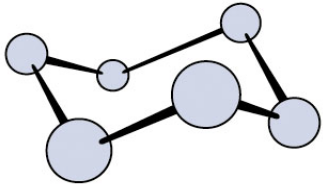
\includegraphics[width=0.6\textwidth]{figures/k16s428S6.png}
\end{flashcard}

\begin{flashcard}[Struktur]{Tegn strukturen af \ce{S8}}
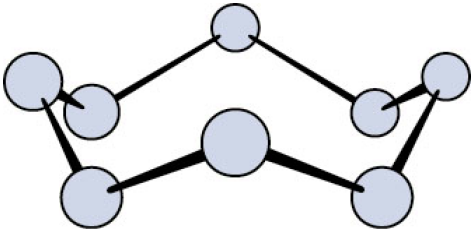
\includegraphics[width=0.6\textwidth]{figures/k16s427S8.png}
\end{flashcard}

\begin{flashcard}[Struktur]{Tegn strukturen af \ce{S12}}
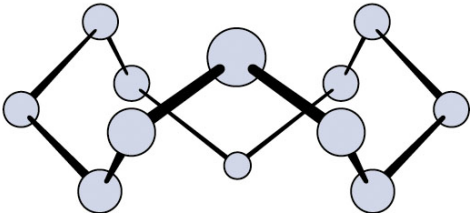
\includegraphics[width=0.7\textwidth]{figures/k16s428S12.png}
\end{flashcard}

\begin{flashcard}[Fremstilling]{Opskriv hvordan man kan fremstille \ce{S6}}
\ce{6Na2S2O3 + 12HCl -> S6(s) + 6SO2 + 12NaCl + 6H2O}
\end{flashcard}

\begin{flashcard}[Fremstilling]{Opskriv hvordan man kan fremstille \ce{S12}}
\ce{H2S8 + S4Cl2 -> S12(s) + 2HCl(g)}
\end{flashcard}

\begin{flashcard}[Fremstilling]{Opskriv reaktionsligninger der beskriver Claus processen}
\ce{2H2S + 3O2 -> 2SO2 + 2H2O}\\
\ce{4H2S + 2SO2 -> 6S(s) + 4H2O}
\end{flashcard}

\begin{flashcard}[Fremstilling]{Angiv hvordan man kan udvinde svovl fra pyrit}
\ce{FeS2 ->[\text{$\Delta$}] FeS + S(s)}
\end{flashcard}

\begin{flashcard}[Reaktion]{Hvordan kan man p�vise sulfid i en vandig opl�sning?}
\ce{Pb(CH3COO)2 + H2S(g) -> PbS + 2CH3COOH}\\ \vspace{7pt}
Blyacetat er farvel�st. Ved reaktion fremkommer sort bly(II)sulfid
\end{flashcard}

\begin{flashcard}[Reaktion]{Hvordan kan man p�vise \ce{SO2} i en vandig opl�sning?}
\ce{Cr2O7^{2-} + 3SO2 + 2H+ -> 2Cr^{3+} + 3SO4^{2-} + H2O}\\ \vspace{7pt}
Dichromat er orange/gult. Ved reaktion skifter opl�sningen farve til gr�n pga. chrom(III) ioner
\end{flashcard}

\begin{flashcard}[Reaktion]{Hvordan kan kraftv�rker oplagre \ce{SO2}?}
\ce{2CaO + 2SO2 + O2 ->[\text{$\Delta$}] 2CaSO4}
\end{flashcard}

\begin{flashcard}[Fremstilling]{Opskriv reaktionsligninger der beskriver trinnene i den industrielle syntese af svovlsyre}
\ce{S + O2 ->[\text{$\Delta$}] SO2}\\
\ce{2SO2 + O2 ->[\text{$\rm V_{2}O_{5}/\Delta$}] 2SO3}\\
\ce{SO3 + H2SO4 -> H2S2O7}\\
\ce{H2S2O7 + H2O -> 2H2SO4}
\end{flashcard}

\begin{flashcard}[Struktur]{Tegn strukturen af \ce{H2SO4}}
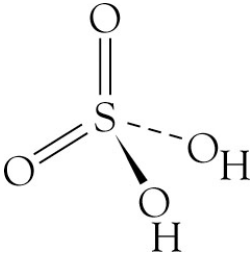
\includegraphics[width=0.4\textwidth]{figures/k16s438H2SO4.png}
\end{flashcard}

\begin{flashcard}[Struktur]{Tegn strukturen af \ce{H2S2O7}}
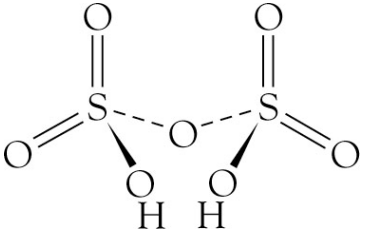
\includegraphics[width=0.7\textwidth]{figures/k16s439H2S2O7.png}
\end{flashcard}

\begin{flashcard}[Reaktion]{Hvad sker der hvis man varmer svovlsyre?}
\ce{2H2SO4 ->[\text{$\Delta$}] 2SO2 + 2H2O + O2}
\end{flashcard}

\begin{flashcard}[Fremstilling]{Angiv hvordan man kan fremstille thiosulfationen}
\ce{SO3^{2-} + S -> S2O3^{2-}}
\end{flashcard}

\begin{flashcard}[Struktur]{Tegn thiosulfationen}
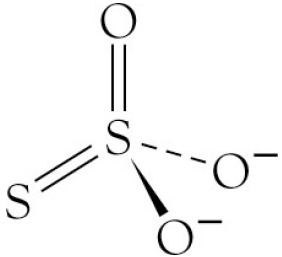
\includegraphics[width=0.5\textwidth]{figures/k16s442S2O32-.png}
\end{flashcard}

\begin{flashcard}[Struktur]{Tegn produktet af elektrolytisk oxidation af thiosulfationen}
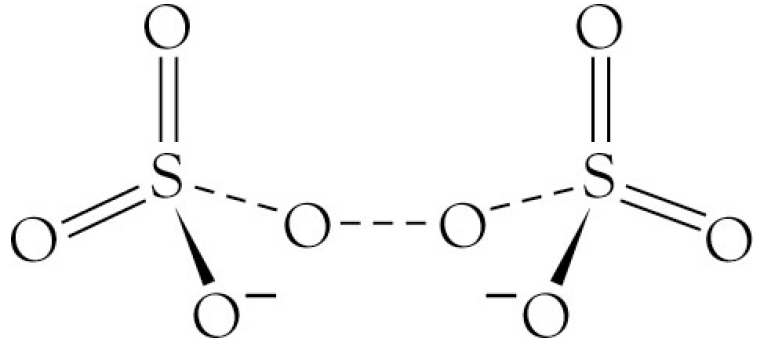
\includegraphics[width=0.7\textwidth]{figures/k16s443Peroxodisulfat.png}
\end{flashcard}

\begin{flashcard}[Fremstilling]{Angiv den simple reaktion for fremstilling af den inerte gas \ce{SF6}}
\ce{S(l) + 3F2(g) -> SF6(g)}
\end{flashcard}

\begin{flashcard}[Struktur]{Tegn strukturen af \ce{S2Cl2}}
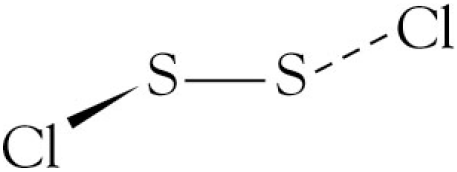
\includegraphics[width=0.7\textwidth]{figures/k16s444S2Cl2.png}
\end{flashcard}